\chapter{Methodology}

To gain insights into the proposed methods for researching the appliance of (ND)-Laplace for cluster algorithms we conducted experiments.
The experiment results are used to evaluate our method against other literature.
In this chapter we explain:
\begin{enumerate}

  \item Datasets
  \item Environmental setup.
  \item For each research question: Description of the different experiments.
  \item For each research question: Results.
\end{enumerate}

\section{Datasets}
For this research, we will use a synthetic dataset for all three research questions.
% Please add the following required packages to your document preamble:
% \usepackage{booktabs}
\begin{table}[h]
  \begin{tabular}{@{}lllll@{}}
    \toprule
    Records & Centers & Dimensions & Standard deviation & Research \\ \midrule
    200     & 4       & 2          & 0.60               & RQ 1     \\ \bottomrule
    200     & 4       & 3          & 0.60               & RQ 2     \\ \bottomrule
    200     & 4       & 5          & 0.60               & RQ 2     \\ \bottomrule
  \end{tabular}
\end{table}

Research question 3 uses a "real-world" dataset to properly assess the different dataset properties that are the subject of this research question.
\todo[inline]{Describe datasets (RQ3)}
\section{Environmental setup}
\todo[inline]{Describe operation system / specs}
\todo[inline]{Describe (python libraries)}
\section{Methods}
This section explains what methods/ algorithms we used and
\subsection{Evaluation}
\todo[inline]{Describe evaluation methodology}
\subsection{Research question 1}

We propose several solutions for open issues based on the theoretical framework. \newline
\subsubsection{Choosing r: } Based, on the idea of chatzikokolakis et al. to lower the size of the radius if the place is crowded, we can do the same with clustering.
For this, we could use a metric like the standard division.
This metric does exactly this, by providing the deviation from the mean:

This metric increases based on clutteredness of the data, which allows us to generate a radius $r$ automatically regardless of domain.
Therefore, we depend on the configurability of epsilon entirely on privacy level $l$.
The generic standard deviation can be defined as:
\begin{equation}
  \sigma = \sqrt{\frac{\sum{(x_i - \mu)^2}}{n}}
\end{equation}
The $\sigma$ being our diameter $d$, the radius $r$ is then calculated as $\frac{d}{2}$. \newline
\subsubsection{Truncation: }
We explained the theory for truncation earlier in paragraph \ref{theory:truncation}.
The methods proposed work correctly for a geographic map where other (historic) locations for remapping are available.

However, it is difficult to apply this to data clustering.
The number of data points is not known beforehand, so we may remap to a location that is too far away.
This way we lose important clusters, which hurts the clustering.
Also, the truncation threshold is so clear (the points are outside the known 2D domain), that we do not have to rely on historical data for remapping.
Our algorithm can be much simpler by re-calculating the noise until it will be within the domain:
\mycomment{
  \begin{equation}
    T(x_{max}, x_{min}, z, x_0) \begin{cases} z &\text{if } 0 < 1 \\ T(x_{max}, x_{min}, planarLaplace(epsilon, x_0), x_0)  &\text{else} \end{cases}
  \end{equation}
}
\begin{algorithm}
  \caption{Truncation algorithm ($T(\min, \max, x_0, z)$) for clustering with planar Laplace}\label{alg:truncaction-rq1}
  \begin{algorithmic}
    \Ensure $z$
    \State $x_1, y_1 \gets x_{min}$
    \State $x_2, y_2 \gets x_{max}$
    \State $z_x, z_y \gets z$
    \If{$x_1 < z_x < x_2$ and $y_1 < z_y < y_2$}
    \State \Return $z$
    \Else
    \State $x, y \gets x_0$
    \State $z_2 \gets LP(\epsilon, x, y)$ \Comment See formula 3.3.
    \State \Return $T(x_{min}, x_{max}, x_0, z_2)$ \Comment Rerun recursively
    \EndIf
  \end{algorithmic}
\end{algorithm}
This algorithm uses $x_{min}$ and $x_{max}$ to re-calculate the points within the domain using respectively the minimum X/Y and maximum X/Y.
An example of this is visualized:
\begin{figure}[h]
  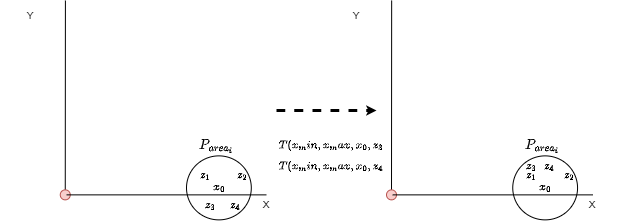
\includegraphics[width=0.8\textwidth]{Method/images/truncation-rq1.png}
  \label{fig:truncation}
  \centering
  \caption{Representation of the remapping algorithm for clustering for points $z_3$ and $z_4$ }
\end{figure}

\subsubsection{Algorithm}
The full algorithm is displayed here.
\begin{algorithm}[H]
  \caption{Full algorithm for perturbing cluster data based on planar/2D-Laplace \citep{DBLP:journals/corr/abs-1212-1984}}\label{alg:rq1}
  \begin{algorithmic}
    \Require $x \in X$  \Comment 2D array of points
    \Require $l \in R^ +$
    \Ensure $z \in Z$ \Comment 2D array of perturbed points
    \State $r = \frac{\sigma}{2}$ \Comment formula 4.1
    \State $\epsilon = \frac{l}{r}$ \Comment Calculating privacy budget \citep{DBLP:journals/corr/abs-1212-1984}
    \State $x_{min} \gets min(X)$
    \State $x_{max} \gets max(X)$
    \State $Z \gets []$
    \For{$point_i \in X$}
    \State $\theta \gets [0, \pi2]$       \Comment Random noise for $\theta$
    \State $p \gets [0, 1]$
    \State $z_i \gets C{_\epsilon}{^{-1}}(p)$       \Comment formula 3.2
    \State $z_i \gets T(x_{min}, x_{max}, point_i, z_i)$ \Comment algorithm 1.
    \State $x_{perturbed} \gets point_{i_x} + (z_{i_x} * \cos(\theta)) $ \Comment add noise to x-coordinate
    \State $y_{perturbed} \gets point_{i_y} + (z_{i_y} * \sin(\theta)) $ \Comment add noise to y-coordinate
    \State append $x_{perturbed}, y_{perturbed}$ to Z
    \EndFor
    \State \Return Z
  \end{algorithmic}
\end{algorithm}
%% We apply the theory for planar laplace proposed by \citep{DBLP:journals/corr/abs-1212-1984}

\subsection{Research question 2}
\subsection{Research question 3}
\section{Results}
\subsection{Research question 1}
\subsection{Research question 2}
\subsection{Research question 3}